\subsection{Experiment 1: The Impact of Estimator Choice and Sample Size on Model Evaluation Reliability}

\begin{figure}[H]
    \centering
    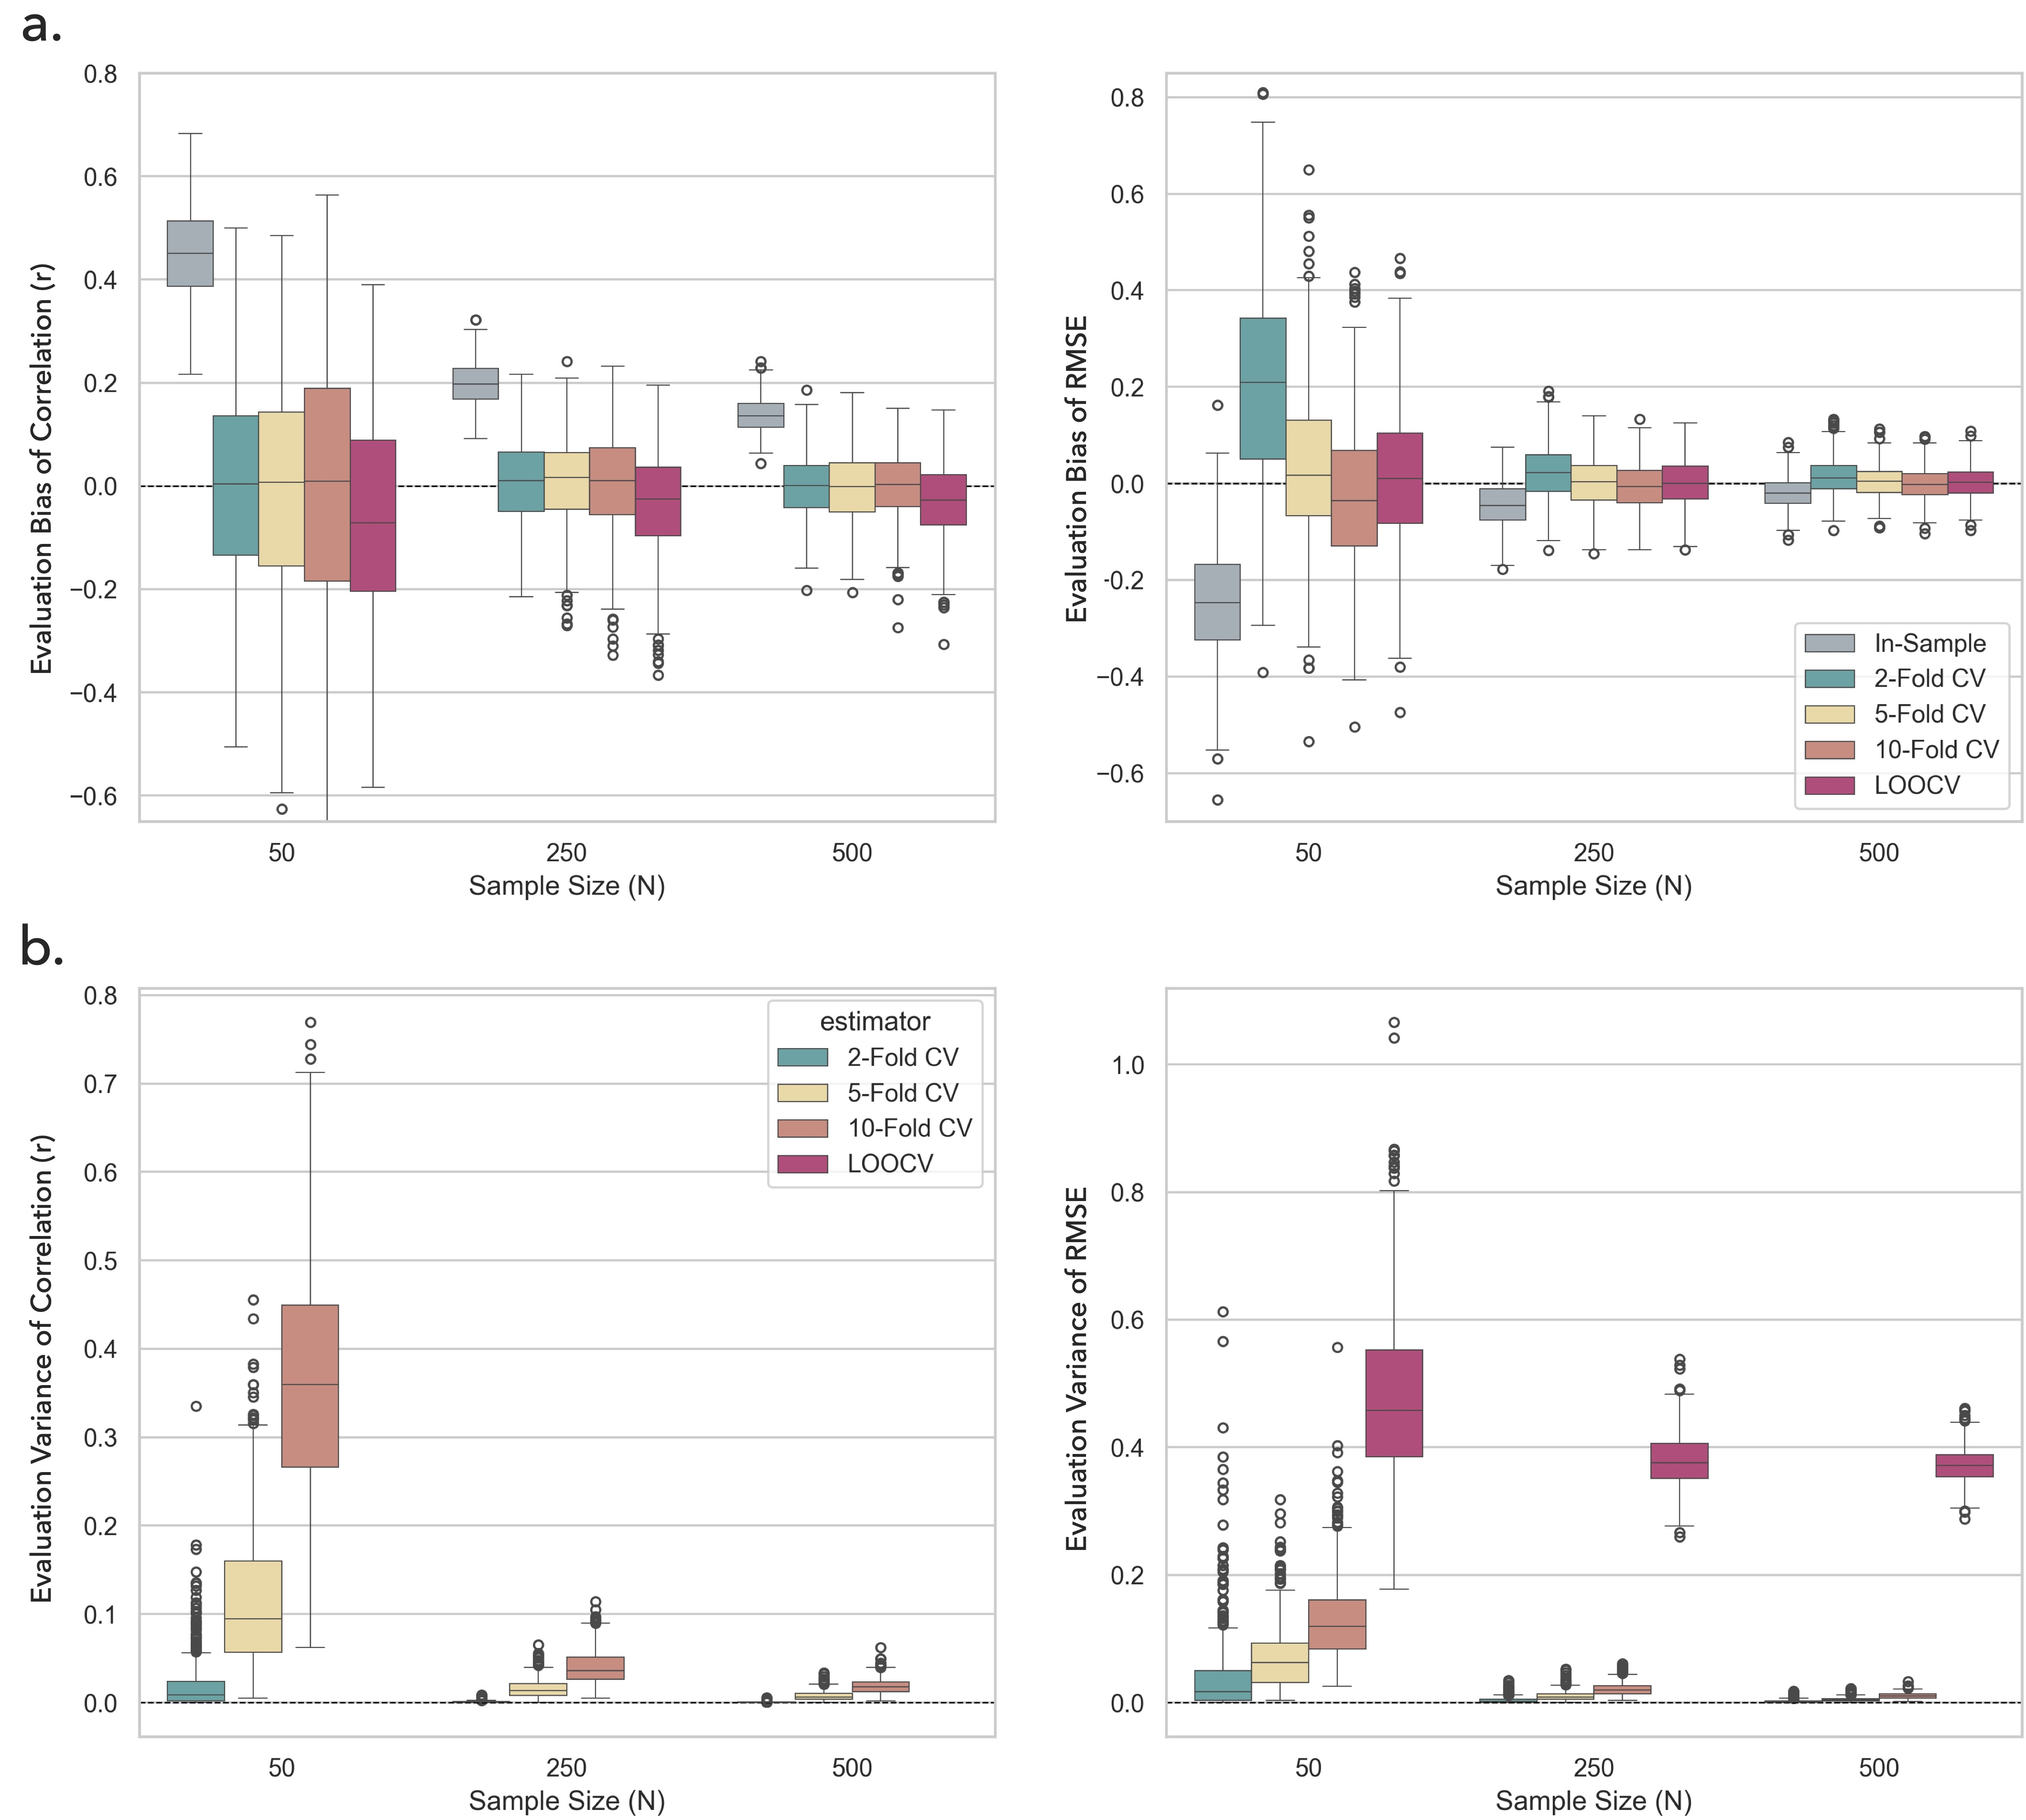
\includegraphics[width=.8\textwidth]{fig_6.jpg}
    \caption{Evaluation bias from 500 sampling iterations on the null dataset with 10 feature variables. Multiple performance estimators across different sample sizes were color-coded. Two metrics: $r$ and RMSE, were displayed in the column facets.}
    \label{fig:s1_biasvar}
\end{figure}


The results (Figure ~\ref{fig:s1_biasvar}, Table ~\ref{tab:eval_bias}, and Table ~\ref{tab:eval_var}) indicate that both the choice of performance estimator and the sample size notably influence evaluation reliability, which can be decomposed into bias and variance. Although different numbers of folds in CV and LOOCV show no substantial differences in bias, they do affect variance. Specifically, as the number of folds increases, the testing sets become smaller, leading to higher variance. Traditionally, LOOCV has been considered an unbiased estimator for error-based metrics such as $R^2$, RMSE, and MAE. In this experiment, LOOCV generally follows that expectation, except for a few cases at certain sample sizes. Interestingly, when the ratio of sample size to number of features is sufficiently high (e.g., 25 when $N=250$), other $K$-fold estimators can deliver comparable accuracy and bias, offering a more computationally efficient alternative to LOOCV.

However, a key finding emerges with correlation-based metrics (e.g., $r$): LOOCV tends to underestimate model performance and exhibits a pessimistic bias. At $N=250$ and $N=500$, LOOCV’s bias on $r$ can be 10 to 30 times larger than other $K$-fold estimators. In contrast, in-sample (or apparent) estimation, while conventionally deemed the most biased due to information leakage from the testing set, can surprisingly achieve comparable reliability at larger sample sizes. For instance, at $N=250$, the bias of in-sample estimation is only 0.099 for $R^2$ and -0.044 for RMSE, which is less biased than all $K$-fold CV estimators for $R^2$ and less biased than 2-fold CV for RMSE with a smaller sample size of 50. Further examination confirms that a higher number of folds in CV generally reduces bias for error-based metrics (RMSE, MAE) because training sets become more representative of the total data. Yet, correlation-based metrics can display divergent trends under the same conditions. In LOOCV, evaluating a single data point at a time makes its variance particularly evident for RMSE, as single-point predictions inherently fluctuate more. Consequently, across all sample sizes tested, LOOCV consistently exhibits greater variance than lower-fold CV (e.g., 2-fold, 5-fold). Nonetheless, bias and variance across all estimators converge as sample size grows (e.g., $N=500$).

Understanding the potential bias associated with each combination of performance estimator and sample size is critical when comparing similar work across multiple studies. For instance, Haque et al. (2023) reported a classification accuracy of 0.991 using 10-fold cross-validation on a dataset of over 3,000 plant leaf images to train a classifier for identifying potential maize diseases \citep{haque_recognition_2023}. The study claimed that its methodology outperformed other works in terms of model performance. However, one of the cited studies reported an accuracy of 0.925, which was based on a dataset of only 100 images and evaluated using a 70/30 train-test split (approximately equivalent to 3-fold cross-validation) \citep{sibiya_computational_2019}. This comparison is therefore worth questioning, as the performance metrics were derived using different evaluation methods and sample sizes. The apparent performance gap may not reflect differences in the models themselves but rather the evaluation strategies employed.

In conclusion, performance estimation reliability depends strongly on the interplay between the estimation method, the metric in use, and the sample size. Larger sample sizes typically reduce both bias and variance, thereby improving the trustworthiness of model evaluations. While LOOCV often provides less biased estimates for error-based metrics, it can severely underestimate correlation-based metrics and suffers from higher variance. $K$-fold CV methods present a more computationally manageable solution for large datasets and can match LOOCV’s performance when the sample size is sufficiently large relative to the number of features. Ultimately, selecting the most appropriate evaluation strategy should be based on practical considerations—such as available sample size, computational resources, and the specific metrics of interest—to ensure robust and reliable model assessments.


\begin{table}[H]
    \caption{Evaluation bias (mean ± std) for the metrics from 500 sampling iterations. The minimum bias given the same sample size is highlighted in bold. N: training sample size; $r$: Pearson correlation coefficient; $R^2$: coefficient of determination; RMSE: root mean squared error; MAE: mean absolute error. CV: cross-validation; LOOCV: leave-one-out cross-validation.}
    \centering
    \begin{tabular}{lcccc}
        \toprule
        \textbf{Metric} & \textbf{Estimator} & \textbf{N=50} & \textbf{N=250} & \textbf{N=500} \\
        \midrule
        \multirow{5}{*}{$r$} 
            & In-Sample
                & 0.449±0.088
                & 0.198±0.043
                & 0.137±0.033 \\
            & 2-Fold CV
                & \textbf{0.004±0.184}
                & 0.009±0.082
                & -0.001±0.061 \\
            & 5-Fold CV
                & -0.012±0.209
                & 0.006±0.088
                & -0.001±0.067 \\
            & 10-Fold CV
                & -0.011±0.254
                & \textbf{0.003±0.094}
                & \textbf{0.000±0.065} \\
            & LOOCV
                & -0.070±0.203
                & -0.035±0.098
                & -0.031±0.071 \\
        \midrule
        \multirow{5}{*}{$R^2$}
            & In-Sample
                & 0.515±0.207
                & 0.099±0.037
                & 0.053±0.020 \\
            & 2-Fold CV
                & -0.694±0.642
                & -0.044±0.071
                & -0.017±0.034 \\
            & 5-Fold CV
                & -0.401±0.409
                & -0.024±0.049
                & \textbf{-0.007±0.026} \\
            & 10-Fold CV
                & -0.940±0.857
                & -0.046±0.052
                & -0.014±0.024 \\
            & LOOCV
                & \textbf{-0.013±0.256}
                & \textbf{0.009±0.039}
                & 0.008±0.020 \\
        \midrule
        \multirow{5}{*}{RMSE}
                & In-Sample
                    & -0.244±0.116
                    & -0.044±0.044
                    & -0.020±0.032 \\
                & 2-Fold CV
                    & 0.215±0.226
                    & 0.022±0.056
                    & 0.013±0.036 \\
                & 5-Fold CV
                    & 0.035±0.158
                    & 0.002±0.047
                    & 0.004±0.033 \\
                & 10-Fold CV
                    & -0.024±0.149
                    & -0.006±0.046
                    & \textbf{-0.001±0.033} \\
                & LOOCV
                    & \textbf{0.012±0.144}
                    & \textbf{0.001±0.046}
                    & 0.003±0.033 \\
        \midrule
        \multirow{5}{*}{MAE}
                & In-Sample
                    & -0.195±0.096
                    & -0.037±0.037
                    & -0.017±0.028 \\
                & 2-Fold CV
                    & 0.180±0.190
                    & 0.017±0.047
                    & 0.010±0.030 \\
                & 5-Fold CV
                    & 0.049±0.134
                    & 0.004±0.039
                    & 0.003±0.028 \\
                & 10-Fold CV
                    & 0.022±0.127
                    & 0.002±0.038
                    & 0.002±0.028 \\
                & LOOCV
                    & \textbf{0.011±0.119}
                    & \textbf{-0.001±0.038}
                    & \textbf{0.001±0.028} \\
        \bottomrule
    \end{tabular}
    \label{tab:eval_bias}
\end{table}
    

\begin{table}[H]
    \caption{Evaluation variance (mean ± std) for the metrics from 500 sampling iterations. The minimum variance given the same sample size is highlighted in bold. N: training sample size; $r$: Pearson correlation coefficient; $R^2$: coefficient of determination; RMSE: root mean squared error; MAE: mean absolute error. CV: cross-validation; LOOCV: leave-one-out cross-validation.}
    \centering
    \begin{tabular}{lcccc}
        \toprule
        \textbf{Metric} & \textbf{Estimator} 
            & \textbf{N=50} & \textbf{N=250} & \textbf{N=500} \\
        \midrule
        \multirow{3}{*}{$r$}
            & 2-Fold CV
                & \textbf{0.019±0.030} 
                & \textbf{0.001±0.001}
                & \textbf{0.000±0.001} \\
            & 5-Fold CV
                & 0.117±0.081
                & 0.016±0.011
                & 0.008±0.005 \\
            & 10-Fold CV
                & 0.362±0.131
                & 0.040±0.019
                & 0.019±0.009 \\          
        \midrule
        \multirow{3}{*}{$R^2$}
            & 2-Fold CV
                & 0.859±2.876
                & \textbf{0.003±0.006}
                & \textbf{0.001±0.001} \\
            & 5-Fold CV
                & \textbf{0.743±1.391}
                & 0.008±0.009
                & 0.002±0.002 \\
            & 10-Fold CV
                & 7.164±37.486
                & 0.018±0.019
                & 0.003±0.002 \\
               
        \midrule
        \multirow{4}{*}{RMSE}
            & 2-Fold CV
                & \textbf{0.041±0.068}
                & \textbf{0.004±0.005}
                & \textbf{0.002±0.003} \\
            & 5-Fold CV
                & 0.070±0.050
                & 0.010±0.008
                & 0.005±0.004 \\
            & 10-Fold CV
                & 0.130±0.067
                & 0.021±0.010
                & 0.010±0.005 \\
            & LOOCV
                & 0.477±0.131
                & 0.379±0.041
                & 0.371±0.029 \\         
        \midrule
        \multirow{4}{*}{MAE}
            & 2-Fold CV
                & \textbf{0.030±0.053}
                & \textbf{0.003±0.003}
                & \textbf{0.001±0.002} \\
            & 5-Fold CV
                & 0.052±0.039
                & 0.008±0.005
                & 0.004±0.003 \\
            & 10-Fold CV
                & 0.100±0.052
                & 0.015±0.007
                & 0.008±0.004 \\
            & LOOCV
                & 0.477±0.131
                & 0.379±0.041
                & 0.371±0.029 \\
        \bottomrule
    \end{tabular}
    \label{tab:eval_var}
\end{table}
